\documentclass[11pt]{article}

% Packages
\usepackage[margin=1in]{geometry}
\usepackage{amsmath, amssymb}
\usepackage{graphicx}
\usepackage{caption}
\usepackage{subcaption}
\usepackage{enumitem}
\usepackage{hyperref}
\usepackage{fancyhdr}
\usepackage{titlesec}

% Header/Footer
\pagestyle{fancy}
\fancyhf{}
\rhead{ML Project Report}
\lhead{Valentin Herrmann, Noah Wedlich}
\cfoot{\thepage}

% Section formatting
\titleformat{\section}{\large\bfseries}{\thesection}{1em}{}
\titleformat{\subsection}{\normalsize\bfseries}{\thesubsection}{1em}{}

% Title
\title{\textbf{Machine Learning Project Report}}
\author{Valentin Herrmann, Noah Wedlich \\
Applied Machine Learning in Python – LMU Munich}
\date{\today}

\begin{document}

% NOTE: specification:
% The report should clearly summarize:
%     What task was addressed
%     How it was approached
%     Why certain methods/experiments were chosen
%     Key results and interpretations
% Include relevant figures (e.g., plots, tables).

\maketitle

\section{Task Overview}
% Briefly describe the dataset or model you worked on, the goal of the project, and why the task is challenging. For example, challenges may include complex preprocessing, large dataset size, class imbalance, poor performance of baseline approaches, or the need for more complex models to achieve good results.

In this project we tested if common models like Kernel SVMs, perceptrons as well as decision tree ensembles suffer from the bias-variance tradeoff. For this purpose we trained and tested the models on simple datasets like concentric bands, interleaving half-moons, spirals and separated Gaussian clusters to produce signs of underfitting and especially of overfitting.
% too slow ⇒ multiprocessing
% getting fitting learning_rate
% creating proper visualizations

\section{Methods}
% Explain the methods you implemented or analyzed. Include relevant equations:

% \[\min_{\mathbf{w}} \quad \frac{1}{2} \|\mathbf{w}\|^2 + C \sum_{i=1}^n \xi_i \]

% Mention any design decisions or implementation notes.
% TunableModel

The implementation of this project can essentially be divided into two parts: the tunable models and the samplers, both of which we will shortly describe here. We chose an object-oriented approach
to allow for easy extension and reuse of the code and to integrate with the Courselib.
\begin{description}
    \item[Tunable Model:] This class provides a convenient way to create and train models on all (or a subset of) the hyperparameter combinations specified. When initialized, it receives
        a subclass of the Courselib \texttt{TrainableModel} class and a dictionary mapping parameter names to their possible values. When training the model, it will instantiate a model
        for each combination of hyperparameters and train it on the given data. Optionally, one can also provide a validator function which can limit the training to a subset of the
        combinations. Since the different models are independent of each other, the training is parallelized using Python's \texttt{multiprocessing} module. We also utilize queues to
        communicate with the main process, which allows us to display the training progress in real-time. If an optimizer is used for training, we will further wrap it to provide
        granular progress updates.
    \item[Samplers:] The samplers are used to generate the datasets on which the models are trained. The subclasses provided here will sample from a distribution on $S\times L\subseteq [-1, 1]^2\times \mathbb{N}$
        where $S$ is some 2D shape and $L$ is a set of labels. The Samplers also provide methods to apply pre- and postprocessing to the data, which can be used to transform the data into a suitable format for training
        and to apply transformations to the data after sampling. This allows to easily test the robustness of models using domain shifts or label noise.
\end{description}

\section{Experiments and Results}
% Present your results. Use figures, tables, and metrics:

In this project, we focused on Kernel SVMs with the RBF kernel, Perceptrons, and Random Forests. We chose a complexity-parameter for each model and repeatedly trained the models
at different complexities. We then used several metrics to analyze the results for signs of over- and underfitting.

\subsection{Perceptrons}
We first considered (multilayer) Perceptrons, i.e. fully connected feedforward neural networks, with the ReLU activation function. We chose the number of hidden layers and the number of neurons per layer as the complexity parameters, as they control the capacity of the model to learn complex functions. We varied these parameters one-by-one to isolate their effects on the model's performance. First we fixed the number of neurons per layer to $30$ and varied the number of hidden layers between $2$ and $16$, the results of which can be seen in Figure~\ref{fig:perceptron_results_layers}.\begin{figure}[h]
    \centering
    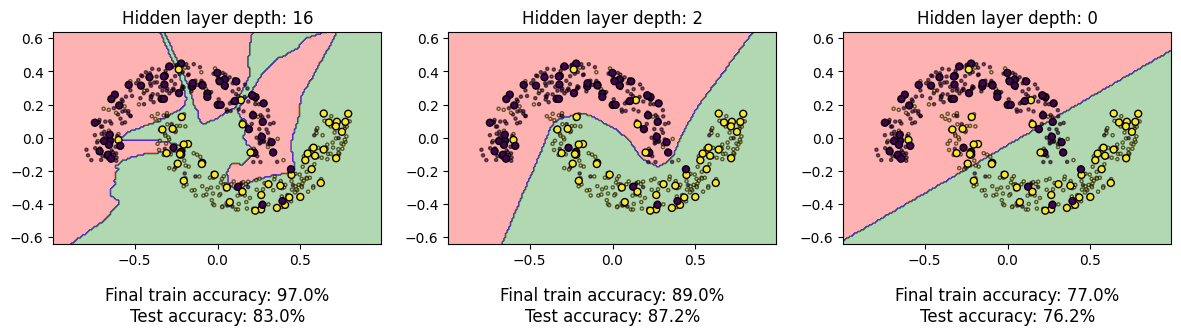
\includegraphics[width=0.8\textwidth]{img/perceptron-depth-result.png}
    \caption{Perceptron results with varying number of hidden layers.}
    \label{fig:perceptron_results_layers}
\end{figure}\\
As can be seen, the training accuracy increases with the number of hidden layers as the model can learn more complex patterns. However, the test accuracy, and thus the generalization performance, starts to decrease after a certain point, indicating that the model is overfitting. This also becomes visible in the decision boundaries: the model is first too simple to separate the data, then finds the correct decision boundary, but then starts to overfit, leading to an unnecessarily complex decision boundary. This effect wasn't observed when varying the number of neurons per layer.

\subsection{Kernel SVMs using the RBF kernel}
Next we analyzed Kernel Support Vector Machines (SVMs) with the RBF kernel. We chose the kernel width $\sigma$ as the complexity parameter, as it controls the sensitivity of the model to the data, i.e. how strongly the model will adapt to the training data. We varied $\sigma$ between $0.02$ and $1$ and trained the model on the spirals. Some results of this are shown in Figure~\ref{fig:kernel_svm_results}.\begin{figure}[h]
    \centering
    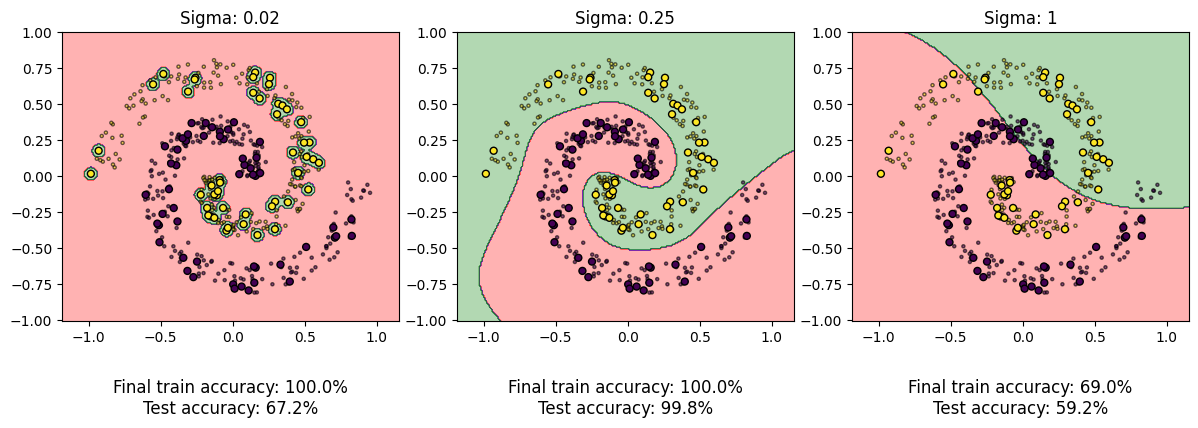
\includegraphics[width=0.7\textwidth]{img/ksvm-result.png}
    \caption{Kernel SVM results with varying kernel width $\sigma$.}
    \label{fig:kernel_svm_results}
\end{figure}\\
These three plots nicely show the three stages of the bias-variance tradeoff. The model on the right is too simple to separate the data, leading to underfitting. The model in the middle is able to separate the data correctly, but the model on the left is too complex and starts to overfit, leading to a drastically worse generalization performance. This also becomes apparent in the decision boundaries, as the model on the left essentially memorizes each training point.

\subsection{Random Forests}
Finally, we considered Random Forests using average voting. We chose both the amount of trees in the ensemble and the maximum tree depth as the complexity parameters. The number of trees controls the amount of noise in the model, while the maximum tree depth controls how complex the individual trees can be. In Figure~\ref{fig:random_forest_results} we show the results of varying the depth, while the effects of varying the number of trees can be seen in the supplementary material.
\begin{figure}[h]
    \centering
    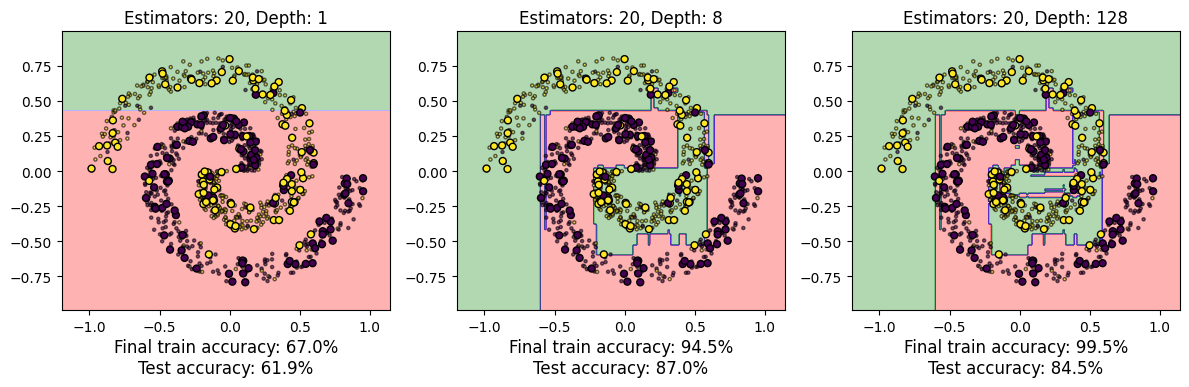
\includegraphics[width=0.7\textwidth]{img/forest-depth-result.png}
    \caption{Random Forest results with varying maximum tree depth.}
    \label{fig:random_forest_results}
\end{figure}\\
These models also exhibit the bias-variance tradeoff, however the overfitting is less pronounced than in the previous models, with the difference in training accuracy being only $2.5\%$.

\subsection{Final Comparison}
Finally we compared the three models on the spirals dataset, using the same complexity parameters as before. The results can be seen in Figure~\ref{fig:final_comparison}. As can be seen, most models follow the same trend, where the training accuracy increases with the complexity, while the test accuracy first increases and then decreases again. The Kernel SVMs are the most sensitive to this effect, as they are less reliant on huge models than the Perceptrons and Random Forests.
\begin{figure}[h]
    \centering
    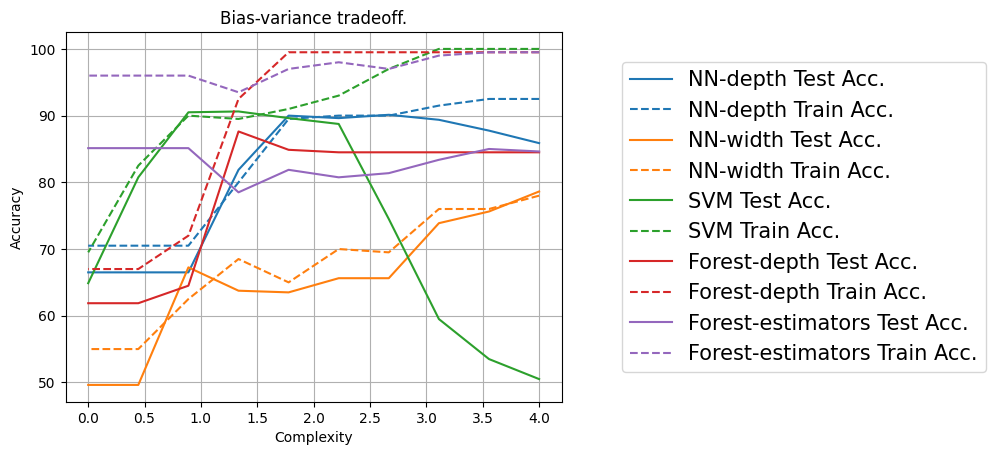
\includegraphics[width=0.6\textwidth]{img/final-result.png}
    \caption{Final comparison of the three models on the noisy spirals dataset.}
    \label{fig:final_comparison}
\end{figure}

% show used data

% \begin{figure}[h]
%     \centering
%     \includegraphics[width=0.5\textwidth]{figures/accuracy_curve.png}
%     \caption{Training/validation accuracy over epochs.}
% \end{figure}

\section{Discussion}
% Summarize key findings, insights, or issues. Optionally, suggest future work or limitations.
We have analyzed the effects of model complexity on the performance of different models and found that all models exhibit signs of overfitting, indicating that the bias-variance tradeoff is a fundamental phenomenon in machine learning. The Kernel SVMs were the most sensitive to this effect. However, we believe that the perceptrons would also show more pronounced overfitting with larger model architectures, something we plan to investigate in the future. 

\end{document}
